\documentclass[10pt]{beamer}
\usepackage[utf8]{inputenc}
\usepackage{amsmath, amssymb, amsthm}
\usepackage{booktabs}
\usepackage{graphicx}

% Theme selection
\usetheme{Madrid}
\usecolortheme{beaver}

% Title slide information
\title{Ridge Regression on Diamonds Dataset}
\subtitle{Comparative Analysis of Optimization Algorithms}
\author{Davide Gamba - Matr 1053470}
\date{\today}

\begin{document}

\begin{frame}
    \titlepage
\end{frame}

\begin{frame}{Introduction}
    The primary objective of this study is to conduct a comparative analysis of the convergence behavior of various optimization algorithms applied on a Ridge Regression problem to the Diamonds Dataset.
    
    \vspace{0.3cm}
    In particular, the focus is on:
    \begin{itemize}
        \item Evaluating the respective algorithms convergence rates.
        \item Investigating how theoretical properties of the objective function (such as Smoothness and Strongly Convexity) have an impact to results.
        \item Evaluating how the $L_2$ regularization parameter ($\lambda$) of Ridge Regression influences speed and efficiency of the algorithms.
    \end{itemize}
    
    \vspace{0.3cm}
    The following algorithms were implemented:
    \begin{itemize}
      \item Gradient Descent (Naive, Bounded, Smooth). 
      \item Accelerated Gradient Descent (Nesterov's).
      \item Stochastic Gradient Descent (Naive, Strongly Convex)
      \item Newton's Method.
      \item Adagrad.
    \end{itemize}

\end{frame}

\begin{frame}{Dataset Overview: The Diamonds Dataset}
    To evaluate the performance of the optimization algorithms, we utilized the \textbf{Diamonds Dataset}. The dataset consists of approximately \textbf{54,000 observations} ($n=53,940$), each representing a diamond with \textbf{10 distinct attributes}.
    
    The primary objective is to predict with a Ridge Regression the \textbf{Price} of a diamond based on its physical and quality characteristics.
    
    \vspace{0.3cm}
    \textbf{Feature Description:}
    \begin{itemize}
        \item \textbf{Target Variable ($y$):} \texttt{price} in US dollars.
        \item \textbf{Numerical Features:} 
        \begin{itemize}
            \item \texttt{carat}: Weight, the most significant predictor.
            \item \texttt{x}, \texttt{y}, \texttt{z}: Length, Width, and Depth in mm.
            \item \texttt{depth}: Total depth percentage ($z / \text{mean}(x, y)$).
            \item \texttt{table}: Width of the top relative to the widest point.
        \end{itemize}
        \item \textbf{Categorical Features (Ordinal):} \texttt{cut}, \texttt{color}, and \texttt{clarity}.
    \end{itemize}
\end{frame}

\begin{frame}{Dataset Overview: The Diamonds Dataset}
  Distribution of all the main variables within the diamonds dataset.
  \vspace{0.3cm}
    \begin{figure}
        \centering
        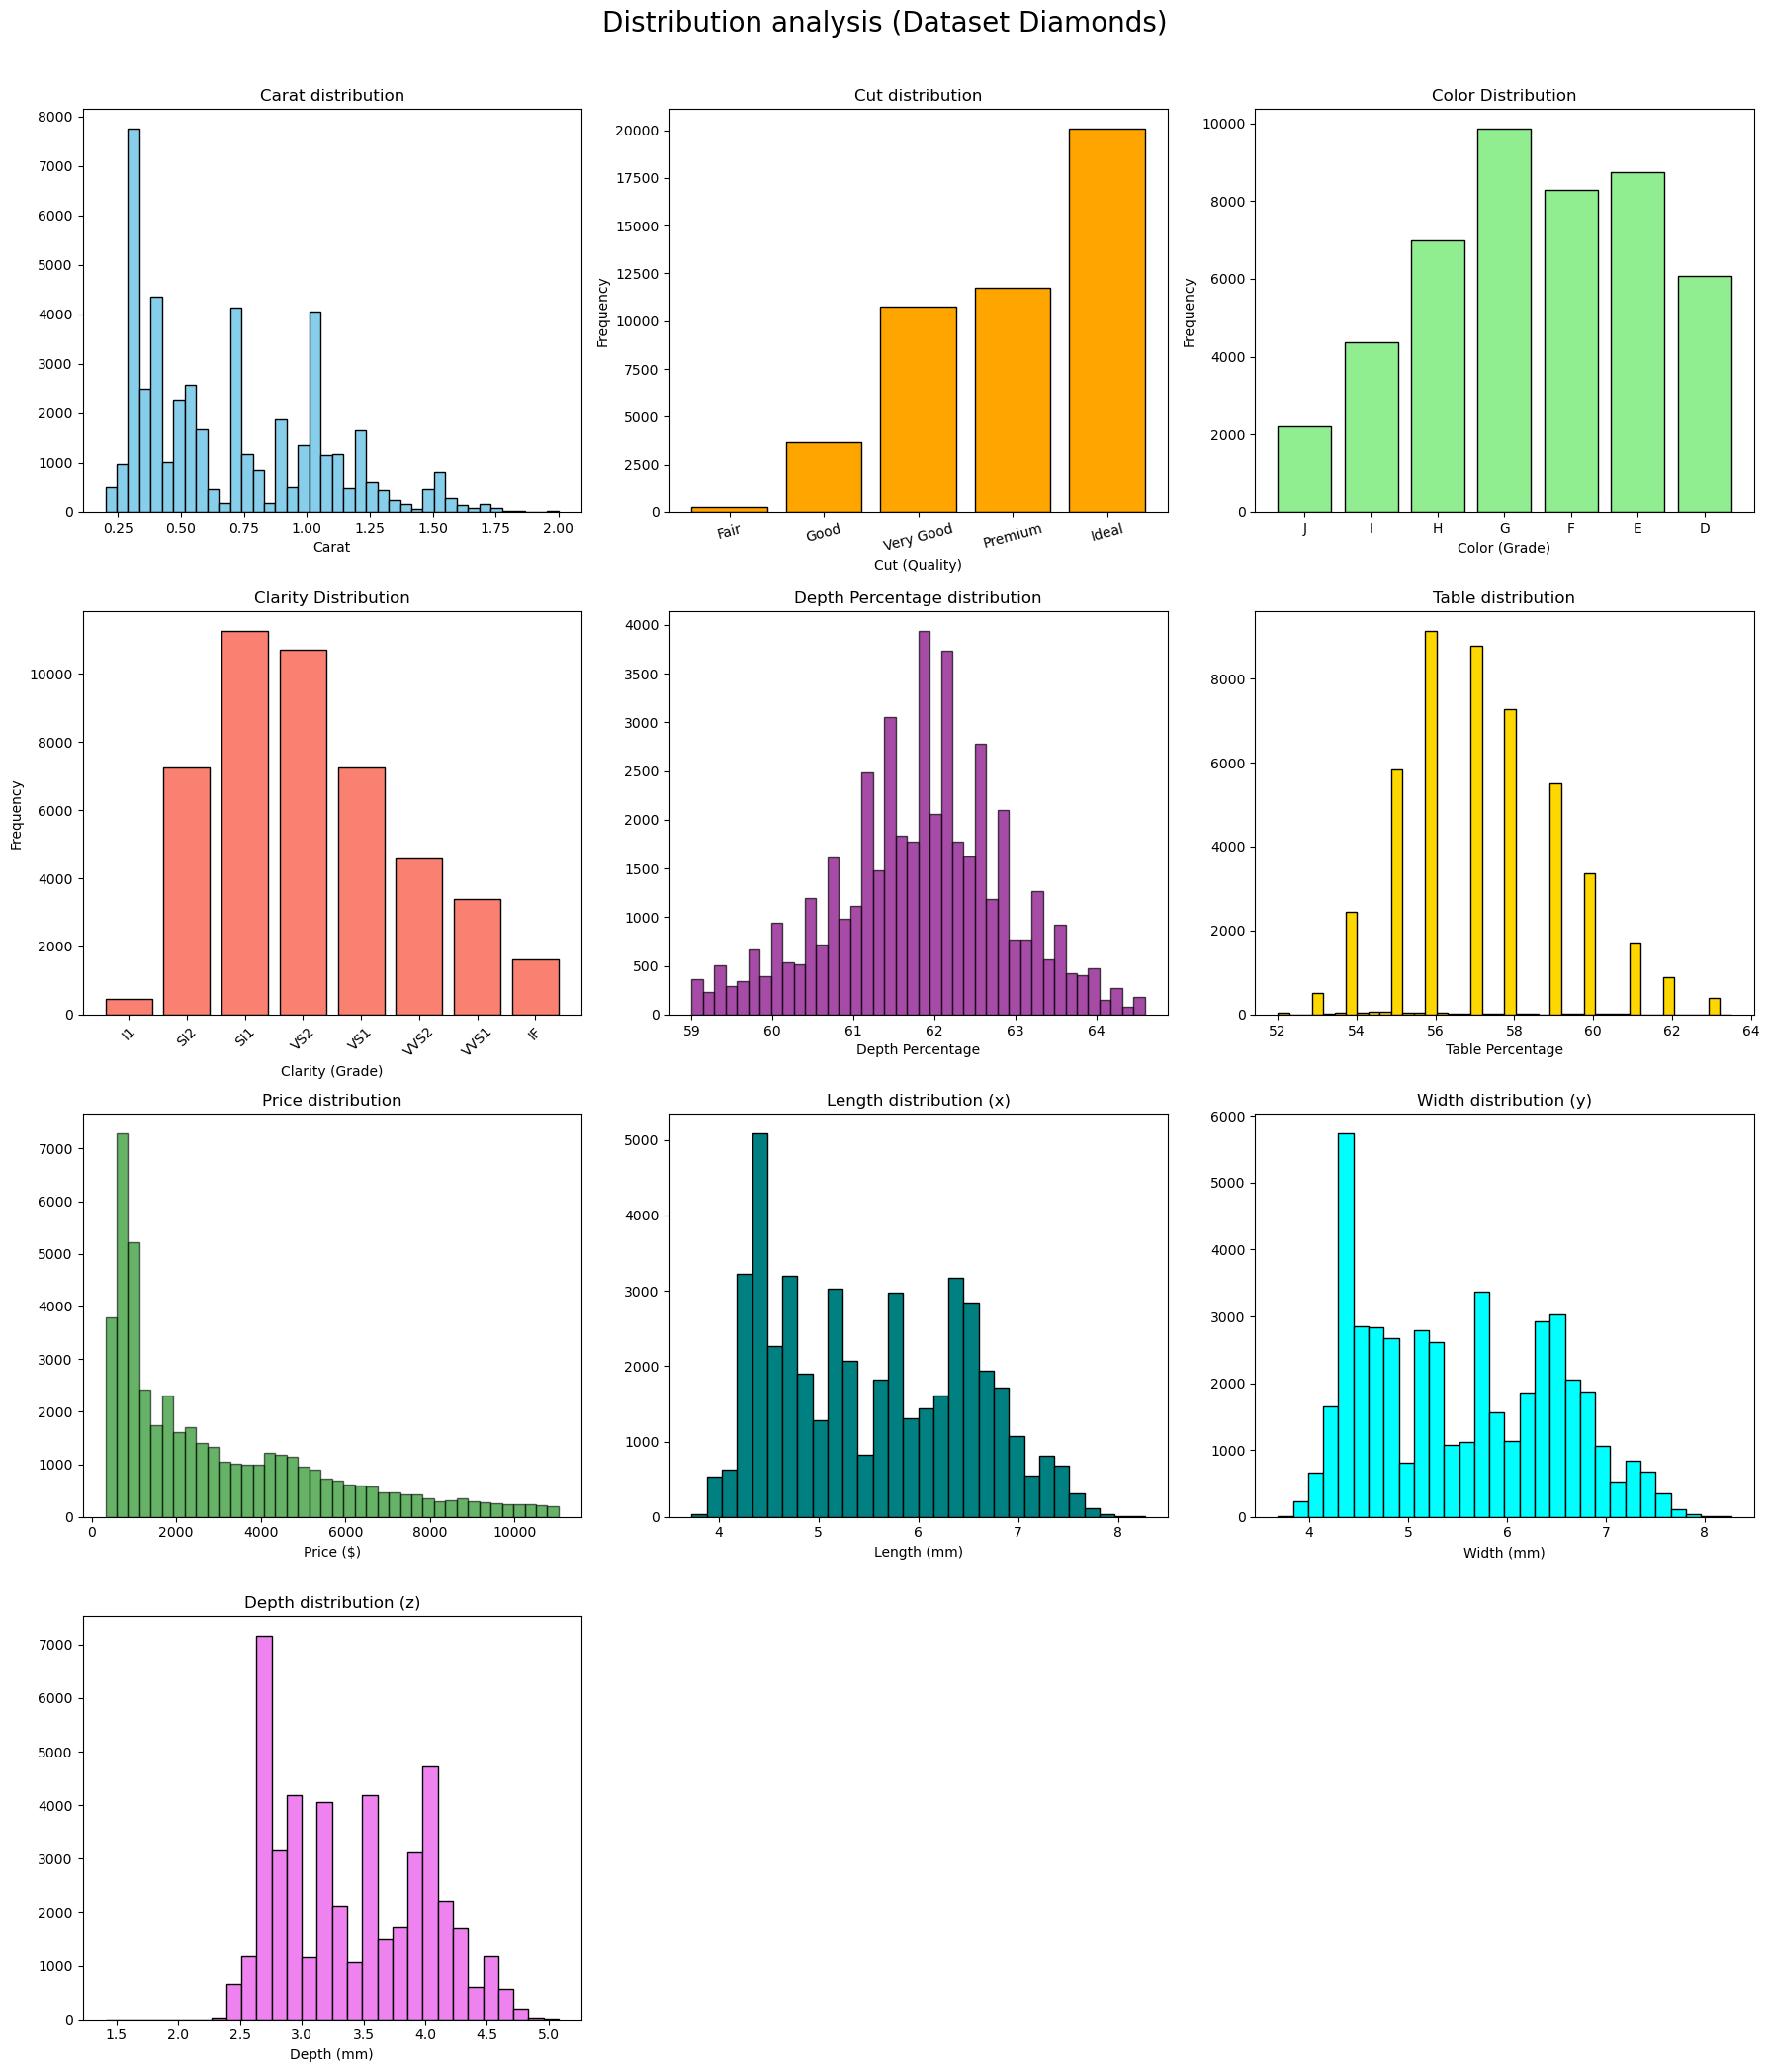
\includegraphics[width=0.8\textwidth,height=0.75\textheight,keepaspectratio]{../images/feature-distribution.png}
    \end{figure} 
\end{frame}

\begin{frame}{Dataset Characteristics: Multicollinearity}
    \textbf{What is Multicollinearity?} \\
    It occurs when two or more independent variables in a regression model are highly linearly correlated, meaning one feature can be accurately predicted from the others.
    
    \vspace{0.3cm}
    \textbf{The Diamonds Case:} \\
    In our specific dataset, there is a strong correlation between \texttt{carat} (weight) and the physical dimensions (\texttt{x}, \texttt{y}, \texttt{z}). These features provide almost identical information.
    
    \vspace{0.3cm}
    \textbf{Impact on Optimization:}
    \begin{itemize}
        \item This structural redundancy results in a feature matrix $X$ with a very small minimum eigenvalue ($\lambda_{\min} \approx 0$).
        \item Consequently, the underlying optimization problem becomes highly \textbf{ill-conditioned}. It is particularly challenging for standard gradient-based methods because it creates flat, unstable valleys in the loss landscape.
    \end{itemize}
\end{frame}

\begin{frame}{Ridge Regression}
    In this study, we address the \textbf{Ridge Regression} problem, which extends Ordinary Least Squares (OLS) by imposing an $L_2$ penalty on the model parameters to mitigate overfitting and multicollinearity.

    \vspace{0.1cm}

    The objective function is the sum of squared errors for each data point ($i=1$ to $n$) plus the sum of squared weights (from $j=1$ to $d$).

    $$f(w) = \frac{1}{2n} \sum_{i=1}^{n} (y_i - x_i^T w)^2 + \frac{\lambda}{2} \sum_{j=1}^{d} w_j^2$$

    The objective function $f(w)$ is defined in vector notation as follows.

    $$
    f(w) = \underbrace{\frac{1}{2n} \| y - Xw \|^2}_{\text{Half MSE}} + \underbrace{\frac{\lambda}{2} \| w \|^2}_{\text{Regularization}}
    $$

    Where:
    \begin{itemize}
        \item $X \in \mathbb{R}^{n \times d}$ is the feature matrix (standardized, includes a column of 1).
        \item $y \in \mathbb{R}^n$ is the target vector (price).
        \item $w \in \mathbb{R}^d$ is the vector of weights to be optimized.
        \item $\lambda > 0$ is the regularization hyperparameter.
    \end{itemize}
\end{frame}

\begin{frame}{Ridge Regression: Why the scaling?}
    \textbf{Why the scaling?}
    
    Introducing specific scaling factors is convenient for mathematical and numerical stability:
    
    \vspace{0.3cm}
    \begin{itemize}
        \item \textbf{The factor $\frac{1}{2}$}: Cancels out the exponent $2$ when computing the gradient $\nabla f(w)$ and the derivative of $\|w\|^2$, simplifying to a linear form without constant multipliers.
        
        \vspace{0.3cm}
        \item \textbf{The factor $\frac{1}{n}$}: Normalizes the error term with respect to the dataset size. This ensures that the magnitude of the loss (and consequently the gradient) is independent of the number of samples $n$. This allows the same learning rates to be effective regardless of whether we use the full dataset or a smaller subset.
    \end{itemize}
\end{frame}

\begin{frame}{Gradient and Hessian Matrix}
    Since $f(w)$ is differentiable, we can work with first-order derivative (the Gradient) and second-order derivative (the Hessian matrix) to minimize the objective function.

    \vspace{0.3cm}
    \textbf{The Gradient $\nabla f(w)$}
    
    The gradient represents the steepest ascent direction of the function. 
    To find the minimum, optimization algorithms like Gradient Descent move in the opposite direction of the gradient. 
    
    Let's expand the vector notation of the objective function:
    $$
    f(w) = {\frac{1}{2n} \| y - Xw \|^2} + {\frac{\lambda}{2} \| w \|^2}
    $$

    $$f(w) = \frac{1}{2n} (y - Xw)^T (y - Xw) + \frac{\lambda}{2} w^T w$$
\end{frame}

\begin{frame}{The Gradient $\nabla f(w)$}
    \small
    Let's expand the error quadratic term:
    $$
    \begin{aligned}
    (y - Xw)^T (y - Xw) &= (y^T - (Xw)^T)(y - Xw) \\
    &= (y^T - w^T X^T)(y - Xw) \\
    &= y^T y - y^T X w - w^T X^T y + w^T X^T X w
    \end{aligned}
    $$

    The terms $y^T X w$ and $w^T X^T y$ are scalars (yielding a $1 \times 1$ result). 
    In linear algebra, the transpose of a scalar is the scalar itself. 
    So $(y^T X w)^T = w^T X^T y$. 
    Therefore, these two terms are identical and can be combined:
    $$- y^T X w - w^T X^T y = -2 w^T X^T y$$

    Now we substitute all in the original function:
    $$
    f(w) = \frac{1}{2n} \left( y^T y - 2 w^T X^T y + w^T X^T X w \right) + \frac{\lambda}{2} w^T w
    $$
\end{frame}

\begin{frame}{The Gradient $\nabla f(w)$}
    \small
    The gradient is the vector of partial derivatives with respect to $w$. 
    To compute the gradients and Hessians, we rely on the following standard matrix calculus properties (assuming $w$ and $b$ are column vectors, and $A$ is a symmetric matrix):

    \begin{enumerate}
        \item \textbf{Constant rule:} $\nabla_w (b) = 0$ 
        \item \textbf{Linear form:} $\nabla_w (w^T b) = \nabla_w (b^T w) = b$
        \item \textbf{Jacobian of a linear mapping:} $\nabla_w (A w) = A$ 
        \item \textbf{Quadratic form:} $\nabla_w (w^T A w) = 2Aw$ \textit{(Requires $A$ to be symmetric, i.e., $A = A^T$. In our case, $X^T X$ and $I$ are both symmetric).}
    \end{enumerate}

    Let's apply these rules to each term of $f(w)$:

    \begin{itemize}
        \item[1.] \textbf{Term $y^T y$}: Does not depend on $w$.
           $$\nabla_w (y^T y) = 0$$

        \item[2.] \textbf{Term $-2 w^T (X^T y)$}: Here $b = X^T y$.
           $$\nabla_w \left( \frac{1}{2n} (-2 w^T X^T y) \right) = -\frac{1}{n} \nabla_w (w^T (X^T y)) = -\frac{1}{n} X^T y$$
    \end{itemize}
\end{frame}

\begin{frame}{The Gradient $\nabla f(w)$}
    \small
    \begin{itemize}
        \item[3.] \textbf{Term $w^T (X^T X) w$}: Here $A = X^T X$. Note that $X^T X$ is symmetric.
           $$\nabla_w \left( \frac{1}{2n} w^T X^T X w \right) = \frac{1}{2n} (2 X^T X w) = \frac{1}{n} X^T X w$$

        \item[4.] \textbf{Regularization term: $\frac{\lambda}{2} w^T w$}: Here $A = I$ (identity matrix).
           $$\nabla_w \left( \frac{\lambda}{2} w^T I w \right) = \frac{\lambda}{2} (2 I w) = \lambda w$$
    \end{itemize}

    \vspace{0.3cm}
    \textbf{Gradient Result:}
    
    Summing all the parts together:
    $$
    \nabla f(w) = \frac{1}{n} (X^T X w - X^T y) + \lambda w
    $$
    
    Factoring out common terms, this is also frequently written as:
    $$\nabla f(w) = \frac{1}{n} X^T (Xw - y) + \lambda w$$

    Gradient is a $d \times 1$ vector.
\end{frame}

\begin{frame}{The Hessian Matrix $\nabla^2 f(w)$}
    The Hessian matrix is the derivative of the gradient with respect to $w$ (i.e., the second derivative of the original function). It is a $d \times d$ matrix.

    Let's recall the expression for the gradient:
    $$\nabla f(w) = \frac{1}{n} X^T X w - \frac{1}{n} X^T y + \lambda w$$

    We differentiate each term with respect to $w$. We use the matrix calculus identity $\nabla_w (Aw) = A$:

    \begin{itemize}
        \item[1.] \textbf{Term $\frac{1}{n} X^T X w$}:
        The constant matrix multiplying $w$ is $\frac{1}{n} X^T X$.
        $$\nabla_w \left(\frac{1}{n} X^T X w\right) = \frac{1}{n} X^T X$$
    \end{itemize}
\end{frame}

\begin{frame}{The Hessian Matrix $\nabla^2 f(w)$}
    \begin{itemize}
        \item[2.] \textbf{Term $-\frac{1}{n} X^T y$}:
        This term does not contain $w$ (it is a constant vector).
        $$\nabla_w \left(-\frac{1}{n} X^T y\right) = 0$$

        \item[3.] \textbf{Term $\lambda w$}:
        We can rewrite this as $\lambda I w$. The constant matrix is $\lambda I$.
        $$\nabla_w (\lambda I w) = \lambda I$$
    \end{itemize}

    \vspace{0.3cm}
    We put the together, so the \textbf{Hessian Matrix} is :
    $$
    H = \nabla^2 f(w) = \frac{1}{n} X^T X + \lambda I
    $$
\end{frame}

\begin{frame}{$f(w)$ is strictly convex}
    To investigate the convexity of our objective function, we rely on the formal definition of definite matrices based on their quadratic forms.\\[0.3cm] 
    \textit{A symmetric matrix $M$ is Positive Semi-Definite if $v^T M v \ge 0$ for all vectors $v$, and Positive Definite if $v^T M v > 0$ for all non-zero vectors $v \neq 0$.}\\[0.3cm]

    Let's apply this definition to our Ridge Regression Hessian matrix, $H = \frac{1}{n} X^T X + \lambda I$, by analyzing its quadratic form $v^T H v$ for any arbitrary non-zero vector $v \in \mathbb{R}^d$:

    $$v^T H v = v^T \left( \frac{1}{n} X^T X + \lambda I \right) v$$

    By distributing the multiplication, we get:

    $$v^T H v = \frac{1}{n} v^T X^T X v + \lambda v^T I v$$
\end{frame}

\begin{frame}{$f(w)$ is strictly convex}
    We can rewrite the first term using the property of transposes, $(Xv)^T = v^T X^T$, and the second term using the definition of the squared $L_2$ norm, $v^T v = \|v\|_2^2$:

    $$v^T H v = \frac{1}{n} (Xv)^T (Xv) + \lambda \|v\|_2^2$$

    $$v^T H v = \underbrace{\frac{1}{n} \|Xv\|^2}_{\text{OLS Base}} + \underbrace{\lambda \|v\|^2}_{\text{Ridge Penalty}}$$

    Now, let's evaluate the two components:

    \begin{itemize}
        \item \textbf{The OLS Base:} The squared norm $\|Xv\|^2$ is a squared length, meaning it is always non-negative ($\ge 0$). This proves that the OLS Hessian ($\frac{1}{n} X^T X$) is intrinsically \textbf{Positive Semi-Definite}. However, if features are perfectly collinear, there exist non-zero vectors $v$ where $Xv = 0$. In these cases, the quadratic form equals zero, meaning the loss function has flat valleys with no unique minimum.
    \end{itemize}
\end{frame}

\begin{frame}{$f(w)$ is strictly convex}
    \begin{itemize}
        \item \textbf{The Ridge Penalty:} For any non-zero vector $v \neq 0$, its squared norm $\|v\|^2$ is strictly positive. Since our regularization hyperparameter is strictly positive ($\lambda > 0$), the entire term $\lambda \|v\|^2$ must be strictly greater than zero ($> 0$).
    \end{itemize}

    \vspace{0.3cm}
    Because we are adding a strictly positive term ($\lambda \|v\|^2 > 0$) to a non-negative term ($\frac{1}{n} \|Xv\|^2 \ge 0$), the entire sum is guaranteed to be strictly positive:

    $$v^T H v > 0 \quad \text{for all } v \neq 0$$

    By the mathematical definition, this proves that the Ridge Hessian matrix $H$ is \textbf{Positive Definite}. The $L_2$ penalty mathematically eliminates any flat regions, guaranteeing that the objective function possesses a single, unique global minimum, so that means $f(w)$ is strictly convex.
\end{frame}

\begin{frame}{Ridge Regression - Properties}
    To understand how iterative optimization algorithms will behave on Ridge Regression objective function $f(w)$, we must analyze its properties. 

    \vspace{0.3cm}
    \textbf{1. Convexity: Yes (Strictly Convex)} \\
    As proven in the previous section using the Hessian's quadratic form, the addition of the $L_2$ penalty ensures that the Hessian matrix $H$ is Positive Definite. Therefore, the function is not just convex, but \textbf{strictly convex}. This guarantees that any local minimum is the unique global minimum $w^*$.

    \vspace{0.3cm}
    \textbf{2. Lipschitz Continuous: No (Globally)} \\
    A function $f(w)$ is globally $B$-Lipschitz if its gradients are bounded in magnitude everywhere ($\| \nabla f(w) \| \le B$). 
    Our objective function $f(w)$ is a quadratic function. As the weights $w$ can grow toward infinity, the gradient $\nabla f(w) = \frac{1}{n} X^T (Xw - y) + \lambda w$ also can grows linearly toward infinity. Because the gradient is unbounded over the entire domain $\mathbb{R}^d$, the function itself is \textbf{not globally Lipschitz continuous}.
\end{frame}

\begin{frame}{Ridge Regression - Properties}

    \textbf{3. Smoothness ($L$-smooth): Yes} \\
    It is \textbf{$L$-Smooth}.
    The curvature does not change abruptly; the gradient doesn't oscillate wildly. The function always lies \textit{below} a certain parabola: 

    $$f(y) \le f(x) + \nabla f(w)^T (y - x) + \frac{L}{2} \|x - y\|^2$$

    \begin{itemize}
        \item \textbf{Value of $L$:} It corresponds to the largest eigenvalue of the Hessian matrix (the maximum curvature of the loss landscape).
          $$L = \lambda_{\max}\left(\frac{1}{n}X^T X\right) + \lambda$$
        \item \textbf{Consequence:} This value acts as the absolute \textbf{speed limit} for Gradient Descent. The optimal safe step size is typically $\gamma = \frac{1}{L}$.
    \end{itemize}
\end{frame}

\begin{frame}{Ridge Regression - Properties}
    \small
    \textbf{4. Strong Convexity ($\mu$-strongly convex): Yes} \\
    It is \textbf{$\mu$-Strongly Convex}.
    The curvature is "at least" $\mu$ in every direction. The function always lies \textit{above} the quadratic function:

    \vspace{-0.2cm}
    $$f(y) \ge f(x) + \nabla f(x)^T (y - w) + \frac{\mu}{2} \|x - y\|^2$$
    \vspace{-0.2cm}

    \begin{itemize}
        \item \textbf{Value of $\mu$:} It corresponds to the smallest eigenvalue of the Hessian matrix.
          $$\mu = \lambda_{\min}\left(\frac{1}{n}X^T X\right) + \lambda$$
          
        \item[] \textit{\footnotesize If the feature matrix $X$ is not full-rank, for instance, due to perfectly collinear features, the minimum eigenvalue of the OLS component $\frac{1}{n}X^T X$ is exactly $0$, meaning $\mu = \lambda$. This mathematically proves that without regularization ($\lambda=0$), the problem might not be strongly convex, which would make convergence much slower.}
        
        \vspace{0.2cm}
        \item \textbf{Consequence:} The larger $\mu$ is, the faster the algorithm will converge to the minimum.
    \end{itemize}
\end{frame}

\end{document}